\documentclass[a4paper]{article}

\usepackage[utf8]{inputenc}
\usepackage[T1]{fontenc}
\usepackage[french]{babel}
\usepackage{fullpage}
\usepackage{hyperref}
\usepackage{amsmath}
\usepackage{amssymb}
\usepackage{upgreek}
\usepackage{color}
\usepackage[]{algorithm2e}
\usepackage{stmaryrd}
\usepackage{graphicx}
\usepackage{float}

\title{
    ELEC-H-201 - Electronique\\
    \small Synthèse 2014-2015
}
\author{Florentin \bsc{Hennecker}}
\date{}

\begin{document}
\maketitle
\tableofcontents

\section{Vademecum d'électricité (chapitre 2)}

    \subsection{Notions fondamentales}

    \subsubsection{Schémas}
    \begin{itemize}
        \item La \textit{charge} d'un montage est l'équipement/composant en aval d'un montage
        \item La \textit{source} d'un montage est l'équipement/composant en amont d'un montage
        \item Deux composants sont connectés en \textit{série} s'ils sont parcourus par le même courant
        \item Deux composants sont connectés en \textit{parallèle} s'ils sont soumis à la même ddp
    \end{itemize}

    \subsubsection{Courants et tensions}

    \paragraph{Intensité} L'\textit{intensité} ou le \textit{courant} 
    est le "débit" de charge électrique : $i() = \frac{dq(t)}{dt}$ en ampères. 
    (\textcolor{red}{[A] = [C/s]}) Elle se mesure avec un ampèremètre en série.
    Ses valeurs courantes vont de $10\mu$A à 100mA.\\

    Sur un schéma, les flèches représentent le \textit{courant conventionnel} formé
    de charges positives (dans le sens contraire du sens réel des électrons).

    \paragraph{Tension} La \textit{tension} est un terme flou et peut représenter 
    une force électromotrice, le potentiel d'un noeud ou la ddp aux bornes d'un dipôle.
    Elle se mesure en \textcolor{red}{[V] = [J/C]}) et oscillera dans ce cours entre 
    100$\mu$V à 100V.

    \paragraph{Potentiel} Le \textit{potentiel électrique} en un point vaut l'énergie
    à dépenser pour amener en ce point une charge électrique unitaire (1C) depuis
    un point où, par convention, ce potentiel vaut 0V.

    \paragraph{Masse} La masse est, par convention, le noeud qui vaut 0V. Attention, 
    masse $\neq$ terre! 

    \paragraph{Force électromotrice} La ddp d'une source idéale est appelée \textit{force électromotrice} (fig \ref{fig:fem})

    \begin{figure}[H]
        \begin{center}
            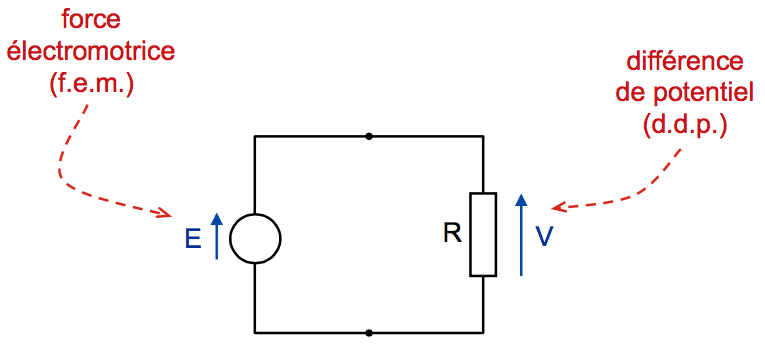
\includegraphics[width=0.6\textwidth]{fig/2_fem.png}
            \caption{Une force électromotrice}
            \label{fig:fem}
        \end{center}
    \end{figure}

    Convention de représentation de la ddp : la flèche de tension pointe vers le
    potentiel le plus positif.

    \paragraph{Charge} La charge se mesure en \textcolor{red}{[C]}). Un électron
    porte une charge élémentaire négative notée $e$, qui vaut environ $-1,6.10^{-19}$C.

    \paragraph{Puissance} La puissance se mesure en \textcolor{red}{[W]}) et
    oscillera dans ce cours entre 10$\mu$W et 10W.

    \subsubsection{Energie et puissance}
    Formule de la puissance instantanée : $$ p(t) = v(t).i(t) $$

    \paragraph{Convention récepteur} Les flèches de courant et de tension sont
    de sens opposés

    \paragraph{Convention générateur} Les flèches de courant et de tension sont
    de même sens\\

    Dans les deux cas, $i>0$ et $v>0$.

    \subsubsection{Etat électrique, loi et caractéristique d'un dipôle}
    L'\textit{état électrique} d'un dipôle est le couple (I,V) de valeurs de
    courant et de tension qui s'appliquent à ce dipôle à un moment donné.

    \paragraph{Loi d'Ohm} $V = R.I$ (aussi appelée loi fondamentale d'un dipôle)

    \paragraph{Caractéristique} La \textit{caractéristique d'un dipôle} est le
    graphe représentant sa loi fondamentale dans le plan (I,V). Le point de fonctionnement
    du dipôle ne peut voyager que sur la caractéristique. \\
    \textbf{Exemple} : la caractéristique d'une source de tension idéale est une
    droite verticale (V constant).

    \paragraph{Résolution} On peut résoudre le circuit soit analytiquement, soit
    graphiquement (intersection des caractéristiques).

    \subsubsection{Principaux dipôles idéaux}
    \paragraph{Résistance} La résistance transforme la puissance électrique reçue
    en énergie thermique. Son unité est l'ohm \textcolor{red}{[$\Omega$]}, et
    oscillera dans ce cours entre $10\Omega$ et $10M\Omega$
    \begin{figure}[H]
        \begin{center}
            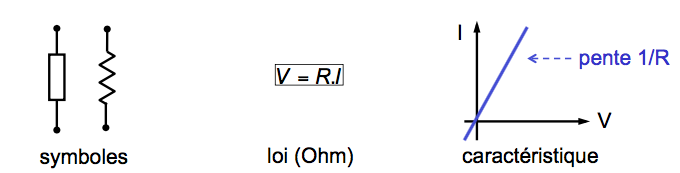
\includegraphics[width=0.6\textwidth]{fig/2_resistance.png}
            \caption{Dipôle résistance}
        \end{center}
    \end{figure}

    \paragraph{Source de tension} Ce dipôle fixe la tension.
    \begin{figure}[H]
        \begin{center}
            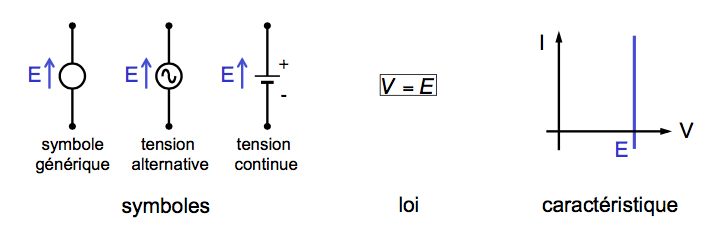
\includegraphics[width=0.6\textwidth]{fig/2_sourcetension.png}
            \caption{Source de tension}
        \end{center}
    \end{figure}

    \paragraph{Source de courant} Ce dipôle fixe le courant.
    \begin{figure}[H]
        \begin{center}
            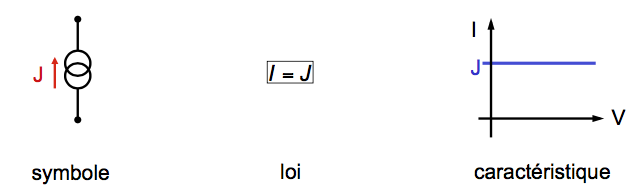
\includegraphics[width=0.6\textwidth]{fig/2_sourcecourant.png}
            \caption{Source de courant}
        \end{center}
    \end{figure}

    \paragraph{Court-circuit} Dipôle dans lequel la tension est nulle.
    \begin{figure}[H]
        \begin{center}
            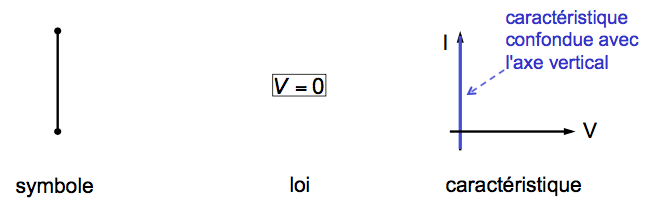
\includegraphics[width=0.6\textwidth]{fig/2_courtcircuit.png}
            \caption{Court-circuit}
        \end{center}
    \end{figure}

    \paragraph{Circuit ouvert} Dipôle dans lequel le courant est nul.
    \begin{figure}[H]
        \begin{center}
            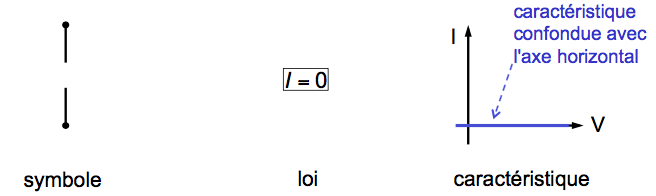
\includegraphics[width=0.6\textwidth]{fig/2_circuitouvert.png}
            \caption{Circuit ouvert}
        \end{center}
    \end{figure}

    \paragraph{Capacité} Sa caractéristique n'est pas représentable sur (I,V) car
    elle fait intervenir la notion de temps. Une capacité s'exprime en farads
    \textcolor{red}{[F]} et oscillera entre 10pF et 1mF.
    \begin{figure}[H]
        \begin{center}
            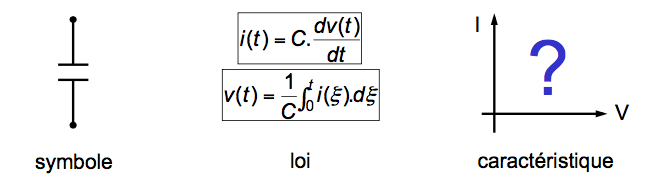
\includegraphics[width=0.6\textwidth]{fig/2_capacite.png}
            \caption{Capacité}
        \end{center}
    \end{figure}

    \paragraph{Inductance} Sa caractéristique n'est pas représentable sur (I,V) non plus.
    Les self-inductances sont exprimées en henris \textcolor{red}{[H]} et oscillent
    entre 10nH et 100mH.
    \begin{figure}[H]
        \begin{center}
            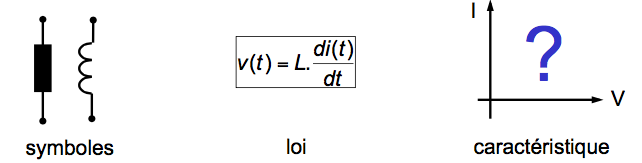
\includegraphics[width=0.6\textwidth]{fig/2_inductance.png}
            \caption{Capacité}
        \end{center}
    \end{figure}

    La capacité et l'inductance ont un statut particulier : elles ne dissipent
    pas de puissance mais sont capables d'emmagasiner de l'énergie et de la 
    restituer ensuite. Ces dipôles sont \textit{réactifs}.\\

    \`A un instant donné, l'énergie accumulée par ces composants vaut : 
    $E = \frac{C.V^2}{2}$ ou $E = \frac{L.I^2}{2}$\\

    \paragraph{Linéarité} On dit qu'un dipôle est \textit{linéaire} si sa caractéristique est une droite.

    \subsection{Equivalent de Thévenin et adaptation d'impédance}

    \subsubsection{Equivalent de Thévenin d'une charge}
    Deux dipôles qui possèdent la même caractéristique sont dits \textit{équivalents}
    (au sens de Thévenin). 

    \paragraph{Exemple} Une résistance de $500\Omega$ et deux résistances de $250\Omega$
    en série.

    \paragraph{Résistance d'entrée} La \textit{résistance d'entrée $R_{in}$} de ce
    dipôle est :
    \begin{itemize}
        \item l'inverse de la pente de la caractéristique de ce dipôle
        \item la valeur de la résistance qui possède la même caractéristique que ce dipôle
    \end{itemize}

    On peut mesurer la résistance d'entrée d'une charge en lui appliquant une tension,
    en mesurant l'intensité du courant entrant dans le dipôle et en faisant
    le rapport entre la tension et le courant. ($R = \frac{V}{I} $)

    \subsubsection{Equivalent de Thévenin d'une source}
    Le problème avec les sources de tensions réelles, c'est que leur caractéristique
    n'est pas entièrement verticale. Leur tension réelle diminue en fait avec
    des intensités de courant plus grandes.\\

    Pour modéliser cette chute de tension, on rajoute une résistance en série
    avec la source de tension idéale. $$V = E - R_{out}.I$$
    \begin{figure}[H]
        \begin{center}
            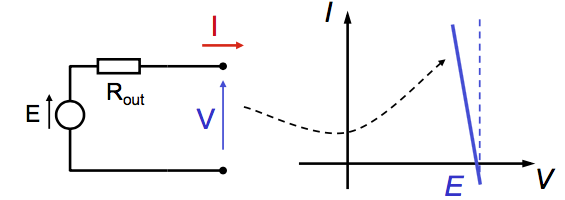
\includegraphics[width=0.6\textwidth]{fig/2_eqtheveninsource.png}
            \caption{Modélisation d'une source de tension réelle}
            \label{fig:2.2.2:eqtheveninsource}
        \end{center}
    \end{figure}

    L'ensemble résistance + source de tension est l'\textit{équivalent de Thévenin}
    de la source réelle. La résistance $R_{out}$ est appelée \textit{résistance
    de sortie}. Tout comme la résistance d'entrée d'une charge, elle est fictive.\\

    La ddp E (sur la fig \ref{fig:2.2.2:eqtheveninsource}) est appelée \textit{
    f.e.m. à vide} car V est égale à E uniquement lorsque la source n'est pas chargée.\\

    On mesure l'équivalent de Thévenin comme suit :
    \begin{itemize}
        \item mesure de la f.e.m. à vide (on place un voltmètre directement à la sortie de la source)
        \item détermination de la résistance de sortie (fig \ref{fig:2.2.2:mesurethevenin}).
    \end{itemize}

    \begin{figure}[H]
        \begin{center}
            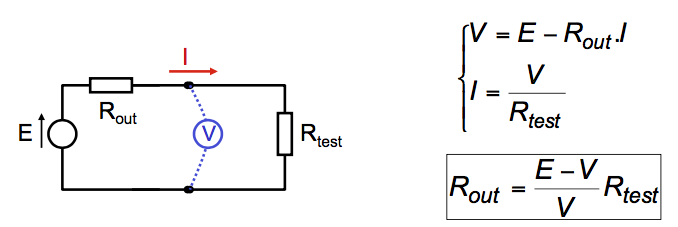
\includegraphics[width=0.6\textwidth]{fig/2_mesurethevenin.png}
            \caption{Détermination de la résistance de sortie}
            \label{fig:2.2.2:mesurethevenin}
        \end{center}
    \end{figure}

    Si $R{test}$ est un potentiomètre, on peut le régler de sorte que la tension
    V vaut la moitié de E $\Rightarrow R_{test} = R_{out}$

    \subsubsection{Théorèmes de Thévenin et de Norton}

    \paragraph{Théorème de Thévenin} Tout dipôle linéaire peut se modéliser
    sous la forme d'un équivalent de Thévenin, où l'équivalent de Thévenin
    est un circuit formé d'une f.e.m. placée en série avec une résistance.\\

    Note : la charge est un cas particulier où il n'y a pas de f.e.m.

    \begin{figure}[H]
        \begin{center}
            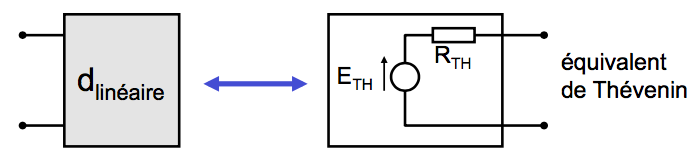
\includegraphics[width=0.6\textwidth]{fig/2_eqthevenin.png}
            \caption{Equivalent de Thévenin}
            \label{fig:2_eqthevenin}
        \end{center}
    \end{figure}

    \paragraph{Théorème de Norton} Tout dipôle linéaire peut se modéliser
    sous la forme d'un équivalent de Norton, où l'équivalent de Norton
    est un circuit formé d'une source de courant placée en parallèle avec une résistance.

    \begin{figure}[H]
        \begin{center}
            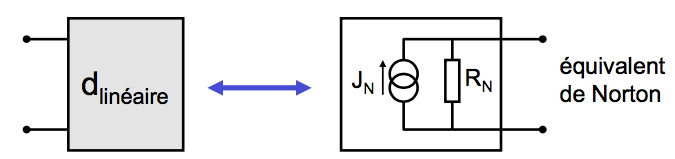
\includegraphics[width=0.6\textwidth]{fig/2_eqnorton.png}
            \caption{Equivalent de Norton}
            \label{fig:2_eqnorton}
        \end{center}
    \end{figure}

    \paragraph{Equivalences} On peut facilement ptasser de l'un à l'autre :
    \begin{align*}
        \begin{cases}
            R_{TH}&= R_N\\
            E_{TH}&= R_N . J_N
        \end{cases}
    \end{align*}

    \paragraph{Dipôles réactifs} Un dipôle réactif ne possède pas de caractéristique
    dans le plan (I,V). Ils possèdent cependant un équivalent de Thévenin (ou Norton).
    Il suffit de remplacer la résistance par une impédance.

    \paragraph{Dipôles non-linéaires} On va obtenir l'équivalent de Thévenin "à petits signaux".
    Il s'agit de l'équivalent de Thévenin de la tangente au point de fonctionnement.
    Cet équivalent n'est donc valable que pour de très faibles variations.

    \subsubsection{Equivalent de Thévenin d'un quadripôle}
    Voici le schéma de l'équivalent de Thévenin d'un quadripôle :
    \begin{figure}[H]
        \begin{center}
            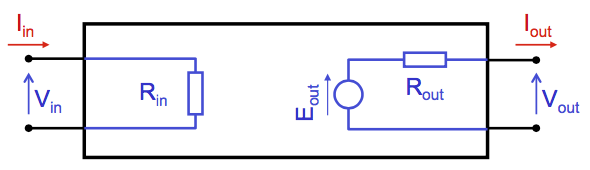
\includegraphics[width=0.6\textwidth]{fig/2_eqtheveninquad.png}
            \caption{Equivalent de Thévenin}
            \label{fig:2_eqtheveninquad}
        \end{center}
    \end{figure}
    On considère en fait l'entrée comme une charge et la sortie comme une source.
    Les conventions récepteur/générateur s'appliquent.

    \paragraph{Source commandée} Dans la fig \ref{fig:2_eqtheveninquad}, si le 
    quadripôle est un ampli, la tension de sortie doit logiquement être $A$ fois
    plus grande que la tension d'entrée. $V_{out}$ dépend de la tension d'entrée
    du quadripôle $V_{in}$ : $E_{out} = A . V_{in}$. Dans ce cas, $E_{out}$ est une 
    source de tension particulière dont la valeur dépend de la tension ou du courant
    en un autre endroit du montage : c'est une \textit{source commandée}.

    \subsubsection{Adaptation d'impédance: cas général}
    \paragraph{Adaptation d'impédance en tension} On considère un appareil amont
    délivrant un signal de tension à un appareil aval. Chacun des appareils
    peut être décrit par son équivalent de Thévenin. Voici comment on peut 
    calculer la tension entre les deux appareils (idée : diviseur résistif)

    \begin{figure}[H]
        \begin{center}
            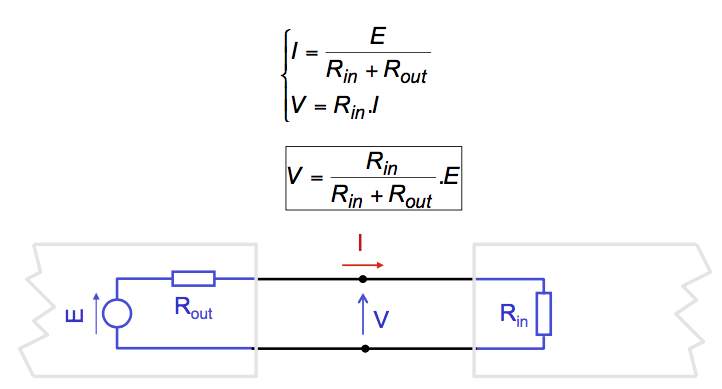
\includegraphics[width=0.6\textwidth]{fig/2_adaptimpedtension.png}
            \caption{Tension reçue par la charge}
            \label{fig:2_adaptimpedtension}
        \end{center}
    \end{figure}

    La tension est donc atténuée d'un facteur $\frac{R_{in}}{R_{in}+R_{out}}$. 
    Il faut donc avoir un $R_{in}$ très élevé ou un $R_{out}$ très faible
    pour limiter la dégradation.

    \paragraph{Critère d'adaptation en tension} Lorsqu'on transmet un signal
    de tension entre deux appareils, il faut une impédance d'entrée élevée
    et une impédance de sortie faible.

    \paragraph{Adaptation d'impédance en courant} Si l'appareil amont se comporte
    davantage comme une source de courant, on utilise l'équivalent de Norton.
    On calcule le courant reçu par l'appareil aval : 
    \begin{figure}[H]
        \begin{center}
            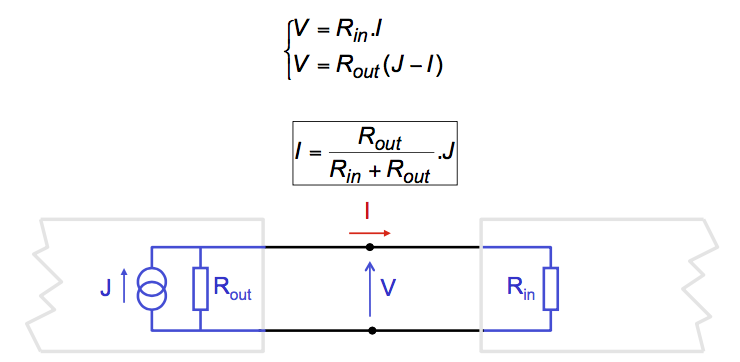
\includegraphics[width=0.6\textwidth]{fig/2_adaptimpedcourant.png}
            \caption{Courant reçu par la charge}
            \label{fig:2_adaptimpedcourant}
        \end{center}
    \end{figure}
    Le courant est effectivement atténué d'un facteur $\frac{R_{out}}{R_{out}+R_{in}}$.

    \paragraph{Critère d'adaptation en courant} Pour éviter une attéunation du courant
    transmis entre deux appareils, il faut une impédance d'entrée faible
    et une impédance de sortie élevée.

    \paragraph{Adaptation d'impédance en puissance}
    \begin{figure}[H]
        \begin{center}
            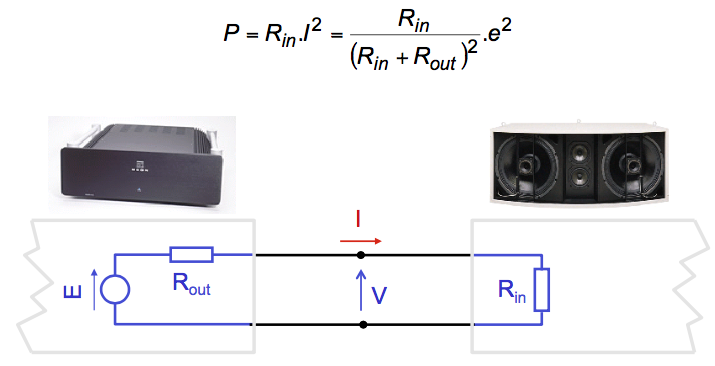
\includegraphics[width=0.6\textwidth]{fig/2_adaptimpedpuissance.png}
            \caption{Puissance reçue par la charge}
            \label{fig:2_adaptimpedpuissance}
        \end{center}
    \end{figure}

    \paragraph{Critère d'adaptation en puissance} On obtient un maximum de puissance
    transmise entre deux appareils lorsque les impédances sont égales. (remarque :
    ce maximum vaut \textbf{la moitié} de la puissance délivrée par l'appareil amont)

    \subsubsection{Application aux instruments de mesure}
    \paragraph{Voltmètre} Modélisé comme une charge, il doit avoir une
    impédance d'entrée beaucoup plus élevée que l'impédance existant entre les 
    noeuds utilisés pour faire la mesure.

    \paragraph{Ampèrementre} Critère classique d'adaptation d'impédance en courant:
    il doit avoir une impédance d'entrée beaucoup plus faible que l'impédance
    existant entre les noeuds utilisés pour faire la mesure.


\end{document}